\section{Baseline: supervised Faster R-CNN}

Allereerst is er een baseline-model nodig om de performance van de andere modellen mee te kunnen vergelijken. Dit model zal op de klassieke manier -- namelijk gesuperviseerd -- getraind worden. Dit houdt in dat het model tijdens het trainingsproces voor elke input een output heeft. Het model kan dus voor elke sample het verband leren tussen de features en de labels. De gesuperviseerde baseline zal daarnaast ook gebruikt worden als backbone voor de andere modellen (cf. infra). \\

In dit onderzoek werden al verschillende populaire supervised objectdetectiemodellen besproken. Hoewel deze allemaal geschikt zijn om als baseline te dienen, zal maar één van deze modellen geïmplementeerd worden. Dit om de simpele reden dat dit slechts een proof of concept is en dat de scope anders te ver zou worden uitgebreid. Het model dat geïmplementeerd zal worden is Faster \gls{rcnn}. De argumenten hiervoor zijn terug te vinden in sectie \ref{sec:modelselectie} van de methodologie.

Er zullen uiteindelijk verschillende varianten van hetzelfde model gebruikt worden in dit onderzoek. De eerste variant is een Faster \gls{rcnn} model dat getraind is op de volledige trainingsset (7600 samples). Deze variant zal gebruikt worden als baseline om de performantie van de andere modellen (\gls{ssl} en \gls{self-sl}) mee te vergelijken. De andere varianten zijn qua architectuur volledig gelijk aan de eerste. Het verschil is dat deze getraind zullen worden op subsets van de trainingsset. Hier wordt dieper op ingegaan in sectie \ref{sec:dataverdeling} van de methodologie. Voor de backbones van de andere leertechnieken zal telkens 5\% en 10\% van de gesuperviseerde data gebruikt worden. Deze modellen zullen daarna gebruikt worden voor de \gls{ssl}- en \gls{self-sl}-modellen. Dit onderzoek zal voor het gesuperviseerde model het experiment in het onderzoek van \textcite{Xie_2022} zo goed mogelijk proberen nabootsen. Aangezien dezelfde dataset gebruikt wordt in dit onderzoek, zullen de resultaten grotendeels hetzelfde zijn. \\

Specifiek zal een Faster \gls{rcnn}-model met een gepretrainde ResNet-18 backbone gebruikt worden. Dit model wordt in het onderzoek van \textcite{Xie_2022} ook gebruikt en heeft een goede performance op de dataset. Zowel het model als de op ImageNet gepretrainde backbone zijn beschikbaar in de TorchVision bibliotheek. Om ze te gebruiken moeten ze enkel geïmporteerd worden, wat onnodig werk en tijd uitspaart ten opzichte van ze zelf te implementeren en volledig opnieuw te trainen. Er wordt gebruikgemaakt van een Adam-optimizer met een \gls{learning_rate} die lineair opgewarmd wordt voor de eerste 500 trainingsstappen. Hierbij wordt de \gls{learning_rate} geleidelijk verhoogd van $1 \times 10^{-4}}$ tot $5 \times 10^{-4}}$. Daarnaast wordt een extra optimalisatie toegepast die ook in de paper voorkomt. Op epoch 8 en epoch 11 wordt de \gls{learning_rate} verminderd met 0.1. In totaal zal er 12 epochs gefinetuned worden. Hierbij wordt geen gebruik gemaakt van de \texttt{EarlyStopping}-callback om de resultaten van de paper zo goed mogelijk na te bootsen. \\

Tijdens het onderzoek werd er ook een poging gedaan om een geoptimaliseerde versie te maken van het trainingsscript. Dit script voerde enkele optimalisaties door die mogelijks de performantie van dit model konden verbeteren. Één van deze optimalisaties was het aanpassen van het vast aantal trainingsstappen waar de lineaire warm-up werd toegepast naar een variabel aantal stappen gebaseerd op een percentage van de hoeveelheid trainingsdata en het aantal epochs. 

\begin{listing}[H]
    \begin{minted}{python}
        total_steps = len(train_loader) * epochs
        warmup_iters = int(total_steps * warmup_pct)
        warmup_iters = max(10, min(warmup_iters, 500))
    \end{minted}
    \caption[Variabele warm-up logica]{Variabele warm-up logica voor het geoptimaliseerd trainingsscript van Faster \gls{rcnn}, gebaseerd op een percentage van de hoeveelheid trainingsdata en het aantal epochs.}
\end{listing}

Daarnaast wordt gebruik gemaakt van een AdamW-optimizer. Dit is betere versie van Adam. Hierbij wordt de \emph{weight decay} ontkoppeld van de update-stap van de gradiënt. AdamW past de \emph{weight decay} namelijk rechtstreeks tijdens de update van de parameters toe. Dit zorgt voor een betere generalisatie en dus een robuuster model. \autocite{Zhou_2024} De \gls{learning_rate} wordt overigens ook opgewarmd van $1 \times 10^{-5}}$ tot $5 \times 10^{-4}}$. De \emph{weight decay} bedraagt $1 \times 10^{-4}}$. Ook wordt gebruik gemaakt van een \texttt{CosineAnnealingLR}-scheduler. Deze scheduler begint met een hoge \gls{learning_rate} en laat deze snel afnemen naar een lage \gls{learning_rate}. \autocite{Loshchilov_2016}. Figuur \ref{fig:cosine_annealing_lr} toont hoe de \gls{learning_rate} evolueert als ook warm-up wordt gebruikt -- zoals in dit script het geval is. In tegenstelling tot het gewone Faster \gls{rcnn}-model, wordt hierbij wel gebruik gemaakt van \texttt{EarlyStopping}. De \gls{map} op een validatieset wordt gemaximaliseerd met een \texttt{patience} van 10 epochs en een \texttt{delta} van 0.001.

\begin{figure}[H]
    \centering
    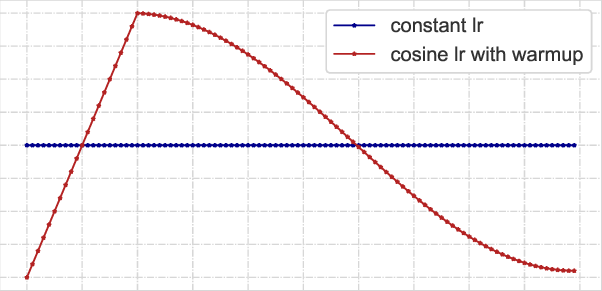
\includegraphics[width=0.7\textwidth]{cosine-annealing-lr-with-warmup.png}
    \caption[Cosine annealing LR]{\label{fig:cosine_annealing_lr}. Vergelijking tussen constante \gls{learning_rate} en \gls{learning_rate} aangepast door een Cosine Annealing LR-scheduler met warm-up. \autocite{Lu_2019}}
\end{figure}

Dit geoptimaliseerd model werd echter niet gebruikt in het uiteindelijke onderzoek om de resultaten zo goed mogelijk met de originele paper van \textcite{Xie_2022} te kunnen vergelijken enerzijds en omdat de performantie van het model ondermaats was anderzijds.